\documentclass{../../oss-classkick-exam}

\begin{document}
\genheader

\gentitle{14}{ELECTROSTATICS}

\genmultidirections

\raggedcolumns
\begin{questions}
  \begin{multicols*}{2}
    \question A positive charge is placed on a spherical conducting hollow shell
    of radius $R$. Which of the following statements is true?
    \begin{choices}
      \choice The charge is distributed evenly on the inside surface of the
      sphere.
      \choice The charge is distributed evenly on the outside surface of the
      sphere.
      \choice The charge is concentrated at the center of the sphere.
      \choice The inside surface of the sphere is negatively charged.
      \choice The charge is concentrated at the poles on the surface of the
      sphere.
    \end{choices}
    \vspace{.7in}
  
%  \question A negative charge is placed on a solid conducting sphere of radius
%  $R$. Which of the following statements is true?
%  \begin{choices}
%    \choice The electric field is zero everywhere inside the sphere.
%    \choice The electric field is zero just outside the surface of the sphere.
%    \choice The electric field is maximum at the center of the sphere.
%    \choice The electric field is directed radially outward outside the surface
%    of the sphere.
%    \choice The electric field inside the sphere is equal and opposite to
%    the electric field outside the surface of the sphere.
%  \end{choices}

    \uplevel{
      \textbf{Questions \ref{cond1}--\ref{cond2}}: A positive charge $Q$ is
      placed at the center of a hollow conducting sphere.
      \begin{center}
        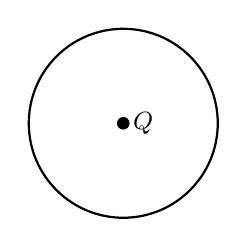
\begin{tikzpicture}
          \draw[thick] circle(1.2);
          \fill circle(.08) node[right]{\small$Q$};
        \end{tikzpicture}
      \end{center}
    }
  
    \question The charge on the inside surface of the hollow sphere is
    \begin{choices}
      \choice $-Q$
      \choice $+Q$
      \choice $-2Q$
      \choice $+2Q$
      \choice zero
    \end{choices}
    \label{cond1}
  
    \question A grounding wire is connected to the sphere, and then removed. The
    charge on the sphere is now
    \begin{choices}
      \choice $-Q$
      \choice $+Q$
      \choice $-2Q$
      \choice $+2Q$
      \choice zero
    \end{choices}
    \label{cond2}
  
    \uplevel{
      \centering
      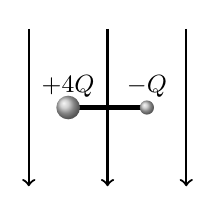
\begin{tikzpicture}
        \foreach\x in {0,1,2}\draw[thick,->](\x,1)--(\x,-1);
        \draw[ultra thick](.5,0)--(1.5,0);
        \shade[ball color=gray!50](.5,0)  circle(.15) node[above]{\small$+4Q$};
        \shade[ball color=gray!50](1.5,0) circle(.09) node[above]{\small$-Q$};
      \end{tikzpicture}
    }
    \question Two charges, $+4Q$ and $-Q$, are connected by an insulated rod and
    rest in a uniform electric field $\vec E$ as shown. Ignore the effects of
    gravity on the charges and rod. The rod and charges will experience
    \begin{choices}
      \choice a clockwise rotation and a downward acceleration
      \choice a counterclockwise rotation and a downward acceleration
      \choice a clockwise rotation and an upward acceleration
      \choice a counterclockwise rotation and an upward acceleration
      \choice no rotation, but a downward acceleration
    \end{choices}
    \vspace{.7in}
  
    \question An electron and a proton are separated by \SI{1.50e-10}\metre. If
    they are released, which one will accelerate at a greater rate, and what is
    the magnitude of that acceleration?
    \begin{choices}
      \choice The electron; \SI{1.12e22}{m/s^2}
      \choice The proton; \SI{1.12e22}{m/s^2}
      \choice The electron; \SI{6.13e18}{m/s^2}
      \choice The proton; \SI{6.13e18}{m/s^2}
      \choice They both accelerate at the same rate; \SI{1.02e-8}{m/s^2}
    \end{choices}
    \columnbreak
  
    \question Four charges are arranged at the corners of a square of side a as
    shown. Which of the following is true of the electric field and the electric
    potential at the center of the square?
    \begin{center}
      \begin{tikzpicture}[scale=1.75]
        \draw[dashed](0,0)--(1,0)--(1,1) node[midway,right]{$a$}
        --(0,1)--cycle;
        \draw[fill=black](.5,.5) circle(0.03);
        \draw[fill=white](0,0) circle(.05) node[below left]{$-q$};
        \draw[fill=white](1,0) circle(.05) node[below right]{$+q$};
        \draw[fill=white](0,1) circle(.05) node[above left]{$+q$};
        \draw[fill=white](1,1) circle(.05) node[above right]{$-q$};
      \end{tikzpicture}
    \end{center}
    \begin{tabular}{rcc}
      & \underline{Electric Field} & \underline{Electric Potential}\\
      (A) & zero & zero \\
      (B) & $\dfrac{kQ}{a\sqrt 2}$ & zero \\
      (C) & $\dfrac{kQ^2}{2a^2}$ &  $\dfrac{kQ}{2a}$\\
      (D) & zero &  $\dfrac{kQ}{\sqrt{2a}}$\\
      (E) & $\dfrac{kQ^2}{2a}$ & $\dfrac{kQ}{a\sqrt 2}$
    \end{tabular}
    \vspace{.7in}
    
    \question Which of the following diagrams best represents how you might
    rearrange the charges so that the electric field at the center would point
    directly toward the top of the page?
    
    \begin{oneparchoices}
      \choice
      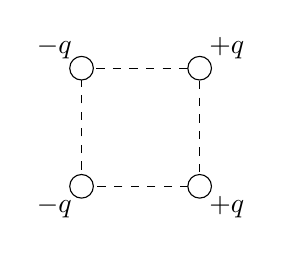
\begin{tikzpicture}[scale=1.5]
        \draw[dashed](0,0) rectangle(1,1);
        \draw[fill=white](0,0) circle(.1) node[below left]{$-q$};
        \draw[fill=white](1,0) circle(.1) node[below right]{$+q$};
        \draw[fill=white](0,1) circle(.1) node[above left]{$-q$};
        \draw[fill=white](1,1) circle(.1) node[above right]{$+q$};
      \end{tikzpicture}
      \choice
      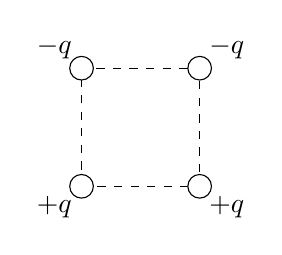
\begin{tikzpicture}[scale=1.5]
        \draw[dashed](0,0) rectangle(1,1);
        \draw[fill=white](0,0) circle(.1) node[below left]{$+q$};
        \draw[fill=white](1,0) circle(.1) node[below right]{$+q$};
        \draw[fill=white](0,1) circle(.1) node[above left]{$-q$};
        \draw[fill=white](1,1) circle(.1) node[above right]{$-q$};
      \end{tikzpicture}
      \choice
      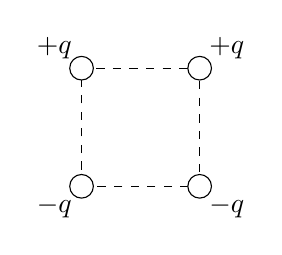
\begin{tikzpicture}[scale=1.5]
        \draw[dashed](0,0) rectangle(1,1);
        \draw[fill=white](0,0) circle(.1) node[below left]{$-q$};
        \draw[fill=white](1,0) circle(.1) node[below right]{$-q$};
        \draw[fill=white](0,1) circle(.1) node[above left]{$+q$};
        \draw[fill=white](1,1) circle(.1) node[above right]{$+q$};
      \end{tikzpicture}
      \choice
      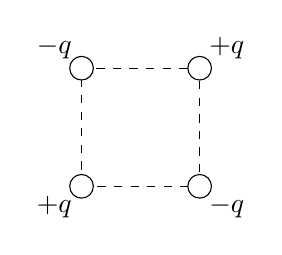
\begin{tikzpicture}[scale=1.5]
        \draw[dashed](0,0) rectangle(1,1);
        \draw[fill=white](0,0) circle(.1) node[below left]{$+q$};
        \draw[fill=white](1,0) circle(.1) node[below right]{$-q$};
        \draw[fill=white](0,1) circle(.1) node[above left]{$-q$};
        \draw[fill=white](1,1) circle(.1) node[above right]{$+q$};
      \end{tikzpicture}
      \choice
      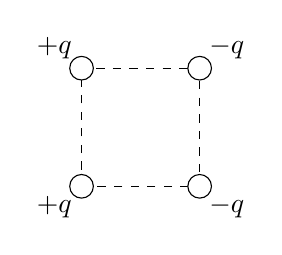
\begin{tikzpicture}[scale=1.5]
        \draw[dashed](0,0) rectangle(1,1);
        \draw[fill=white](0,0) circle(.1) node[below left]{$+q$};
        \draw[fill=white](1,0) circle(.1) node[below right]{$-q$};
        \draw[fill=white](0,1) circle(.1) node[above left]{$+q$};
        \draw[fill=white](1,1) circle(.1) node[above right]{$-q$};
      \end{tikzpicture}
    \end{oneparchoices}
    \vspace{.7in}
    
    \question Three charges, $+Q$, $-Q$, and $+2Q$, are arranged in an
    equilateral triangle as shown. Which of the arrows below best represents the
    direction of the electric field at the center of the triangle?
    \begin{center}
      \vspace{-.1in}
      \begin{tikzpicture}[scale=2]
        \draw[dashed](0,0)--(1,0)--(.5,.866)--cycle;
        \draw (.5,.289) circle(.03);
        \draw[fill=white](0,0)     circle(.05) node[left] {$+Q\;$};
        \draw[fill=white](1,0)     circle(.05) node[right]{$\;-Q$};
        \draw[fill=white](.5,.866) circle(.05) node[above]{$2Q$};
      \end{tikzpicture}
    \end{center}
    \begin{choices}
      \choice {\Huge$\downarrow$}
      \choice {\Huge$\uparrow$}
      \choice {\Huge$\searrow$}
      \choice {\Huge$\swarrow$}
      \choice {\Huge$\nearrow$}
    \end{choices}
    \columnbreak
    
    \question Electric potential
    \begin{choices}
      \choice is a vector quantity that depends on the direction of the electric
      field
      \choice is a scalar quantity that depends on the magnitude and sign of
      charges in the vicinity
      \choice is a scalar quantity that depends on the square of the distance
      from the charges in the vicinity
      \choice is a vector quantity that depends on the sign of the charges in
      the vicinity
      \choice is a vector quantity that must point from high to low potential
    \end{choices}
    \vspace{.7in}
   
    \question A positively charged ring of radius $R$ is made of conducting
    material and has a charge $Q$ distributed uniformly around it. The center of
    the ring is located at point $0$ on the $x$-axis. The potential $V$ at a
    distance $3d$ from point $0$ on the $x$-axis is
    \begin{center}
      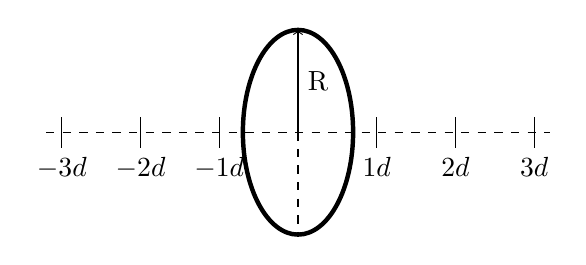
\begin{tikzpicture}
        \draw[ultra thick] (0,0) ellipse (0.7 and 1.3);
        \draw[->](0,0)--(0,1.3) node[midway,right]{R};
        \draw[dashed](0,0)--(0,-1.3);
        \draw[dashed](-3.2,0)--(3.2,0);
        \foreach \x in {-3,-2,-1,1,2,3}{
          \draw(\x,-.2)--(\x,.2) node[pos=0,below] {$\x d$};
        }
      \end{tikzpicture}
    \end{center}
    \begin{choices}
      \choice $V=\dfrac{kQ}{9d^2}$
      \choice $V=\dfrac{kQ}{3d^2}$
      \choice $V=\dfrac{kQ}{R^2+9d^2}$
      \choice $V=\sqrt{\dfrac{kQ}{R^2+9d^2}}$
      \choice $V=\dfrac{kQ}{\sqrt{R^2+9d^2}}$
    \end{choices}
    \columnbreak
  
    \question Which of the following statements is true of electric field and
    equipotential lines?
    \begin{choices}
      \choice The electric field vector always points in the same direction as
      the equipotential lines.
      \choice The electric field always points in the opposite direction of the
      equipotential lines.
      \choice The electric field always points perpendicular to the
      equipotential lines.
      \choice The electric field is always equal to the equipotential lines.
      \choice Equipotential lines always form a circle around electric field
      lines.
    \end{choices}
    \vspace{.7in}
   
    \question The potential $V$ as a function of distance $r$ for a particular
    charge distribution is given by the equation $V=ar^{-1}$. The electric field
    as a function of distance $r$ from the charge distribution is
    \begin{choices}
      \choice $\dfrac13ar^{-3}$
      \choice $2ar^{-1}$
      \choice $ar^{-2}$
      \choice $-a(\ln r)$
      \choice $-ar^{-2}$
    \end{choices}
  \end{multicols*}
  \newpage

  \uplevel{
    \genfreetitle{14}{ELECTROSTATICS}{3}
    \genfreedirections
  }

  \question In the Bohr model of the hydrogen atom, the electron moves in a
  circular orbit of radius $r$ around the proton.
  \begin{parts}
    \part Find an expression for the kinetic energy of the electron as a
    function of $r$. Show that at any distance $r$ the kinetic energy is half
    the potential energy.
    \part Evaluate kinetic energy $K$, potential energy $U$ and the total
    energy $W=K+U$ in electron volts for\\ $r=\SI{0.529e-10}\metre$, the
    radius of the electron's orbit in hydrogen. (The energy $|W|$ that must be
    supplied to the hydrogen atom to remove the electron is called the
    ionization energy.)
  \end{parts}
  \newpage

  % TAKEN FROM 2016 AP PHYSICS C EXAM FREE-RESPONSE QUESTION E&M 1
  \uplevel{
    \cpic{.9}{potentials}
  }
  \question Two point charges, $q_1$ and $q_2$, are fixed in place on the
  $x$-axis at positions $x_1=\SI{-1.00}\metre$ and $x_1=+\SI{0.50}\metre$,
  respectively. Charge $q_2$ has a value of \SI{2.}{\nano\coulomb}. Values of
  electric potential are illustrated by the given equipotentials in the diagram
  shown above, which is drawn to scale.
  \begin{parts}
    \part Calculate the value of $q_1$.
    
    \part At point $C$ on the diagram, draw a vector representing the direction
    of the electric field at that point.
    
    \part Calculate the approximate magnitude of the electric field strength at
    point $D$ on the diagram.
    
    \part The equipotential labeled $\SI0\volt$ is the cross section of a
    nearly spherical surface. Calculate the electric flux for this surface.
    
    \part A proton is placed at point $A$ and then released from rest.
    \begin{subparts}
      \subpart Calculate the work done by the electric field on the proton as it
      moves from point $A$ to point $E$.
      
      \subpart Calculate the speed of the proton when it reaches point $E$.
    \end{subparts}
    
    \part An electron is released from rest at point $B$. Which of the following
    indicates the direction of the initial acceleration, if any, of the
    electron? Justify your answer.

    \vspace{.1in}
    \underline{\hspace{.3in}} Up\hspace{.2in}
    \underline{\hspace{.3in}} Down\hspace{.2in}
    \underline{\hspace{.3in}} Left\hspace{.2in}
    \underline{\hspace{.3in}} Right\hspace{.2in}
    \underline{\hspace{.3in}} Into the page\hspace{.2in}
    \underline{\hspace{.3in}} Out of the page

    \vspace{.1in}\underline{\hspace{.3in}} The direction is undefined since the
    acceleration is zero.
  \end{parts}
  \newpage
  
  \question A spherically symmetric charge distribution has net positive charge
  $Q_0$ distributed within a radius of $R$. Its electric potential $V$ as a
  function of the distance $r$ from the center of the sphere is given by the
  following
  \begin{align*}
    V(r) &= \frac{Q_0}{4\pi\epsilon_0R}\left[-2+3\left(\frac rR\right)^2 \right]
    \text{ for } r<R\\
    V(r) &= \frac{Q_0}{4\pi\epsilon_0r}\text{ for } r>R
  \end{align*}
  Express all algebraic answers in terms of the given quantities and
  fundamental constants.
  \begin{parts}
    \part For the following regions, indicate the direction of the electric
    field $E(r)$ and derive an expression for its magnitude.
    \begin{subparts}
      \subpart $r < R$
      
      \vspace{.1in}\underline{\hspace{.4in}} Radially inward
        
      \vspace{.1in}\underline{\hspace{.4in}} Radially outward
      
      \subpart $r > R$
      
      \vspace{.1in}\underline{\hspace{.4in}} Radially inward

      \vspace{.1in}\underline{\hspace{.4in}} Radially outward
    \end{subparts}
    
    \part For the following regions, derive an expression for the enclosed
    charge that generates the electric field in that region, expressed as a
    function of $r$.
    \begin{subparts}
      \subpart $r < R$
      \subpart $r > R$
    \end{subparts}

    \part Is there any charge on the surface of the sphere ($r=R$)?

    \vspace{.1in}
    \underline{\hspace{.4in}} Yes\hspace{.3in}
    \underline{\hspace{.4in}} No
    
    If there is, determine the charge. In either case, explain your reasoning.

    \part On the axes below, sketch a graph of the force that would act on a
    positive test charge in the regions $r<R$ and $r > R$. Assume that a force
    directed radially outward is positive.
    \begin{center}
      \begin{tikzpicture}[scale=1.1]
        \draw[very thick,->](0,-3)--(0,3) node[above]{$F$};
        \draw[very thick,->](0,0)--(10,0) node[right]{$r$};
        \draw[dashed](4,-3)--(4,3) node[midway,below left]{$R$};
      \end{tikzpicture}
    \end{center}
  \end{parts}
\end{questions}
\end{document}
